\section{Auswertung}
\label{sec:Auswertung}

% \begin{figure}
%   \centering
%   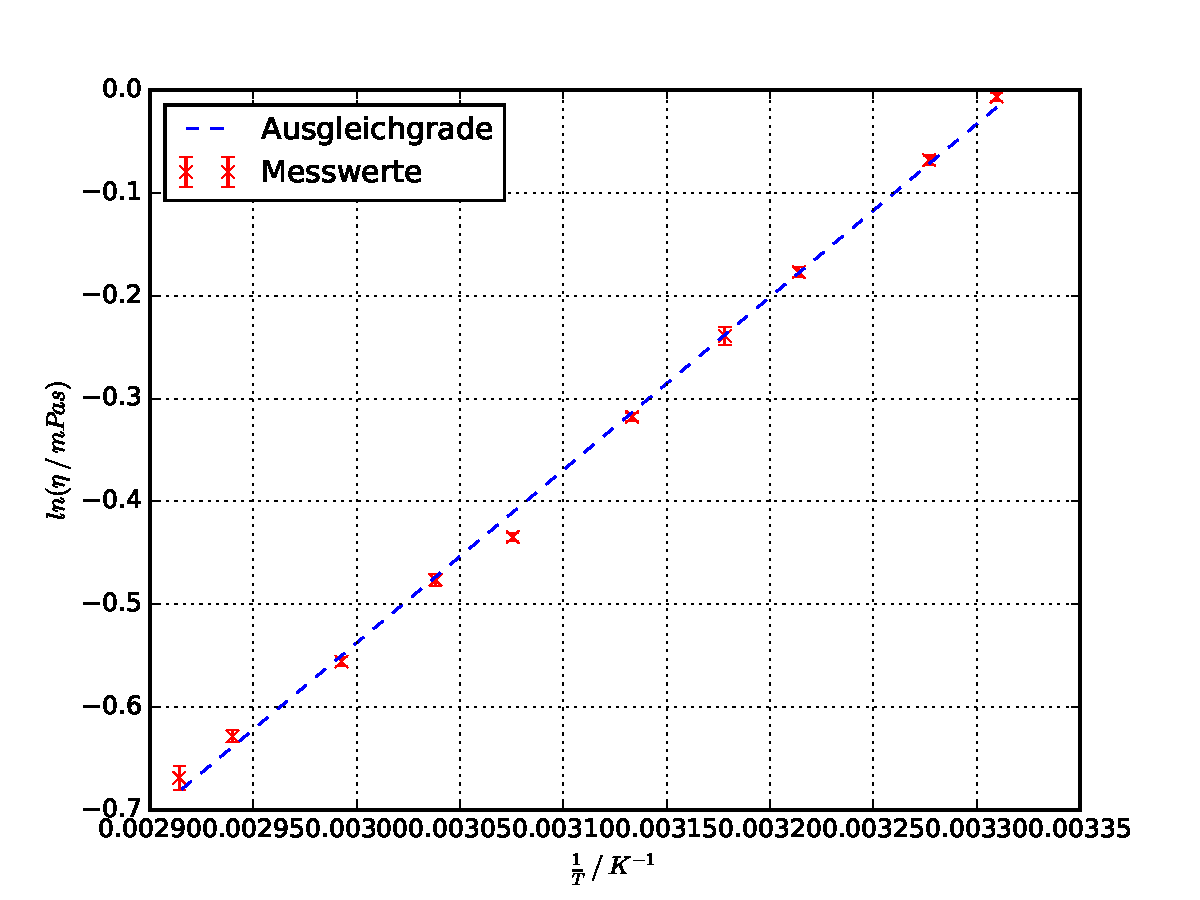
\includegraphics{plot.pdf}
%   \caption{Plot.}
%   \label{fig:plot}
% \end{figure}

\subsection{Methoden}
Alle Mittelwerte und deren Fehler wurden mit den Formeln
\begin{equation}
  \langle x \rangle = \frac{1}{n} \sum_{i=1} ^{n} x_i \quad \text{und} \quad
  \Delta x = \sqrt{\frac{1}{n(n-1)} \sum_{i=1}^n (x_i - \langle x \rangle )^2}
  \label{eqn:MW}
\end{equation}
berechnet \cite{Tipler}.
\subsection{Dampfdruck und die mittlere freie Weglänge}
Die Werte für Dampfdruck und mittlerer freier Weglänge wurden mit den Formeln
\eqref{eqn:p} und \eqref{eqn:Weg} berechnet.
In der Tabelle \ref{tab:ue} sind die Temperturen, Dampfdrücke, mittlere Weglängen
sowie der Größenfaktor $ \sfrac{a}{\bar{w}}$ dargestellt, wobei $a = 1 \si{\centi \meter}$ bei
der verwendeten Versuchapparatur beträgt. Die Tabelle zeigt die Werte zweilenweise für
die verschieden Versuchsteile, d.h. die ersten beiden Zeilen zeigen die Werte für
die Messung der integralen Energieverteilung bei verschiedenen Temperturen, die Dritte
für die Messung der Franck-Hertz-Kurve und die vierte für die Messung der Ionisierungsspannung.
Der Größenfaktor sollte zischen 1000 und
4000 liegen, da sonst keine ausreichend große Stoßwahrscheinlichkeit gewährleistet ist.
Aus der Tabelle \ref{tab:ue} ist also zu entnehmen, dass nur bei der Messung
der integrale Energieverteilung eine ausreichende
Stoßwahrscheinlichkeit gewährleitstet war und bei der Messung der Franck-Hertz-Kurve
wesentlich zu hoch war.

\begin{table}
  \centering
  \caption{Temperaturen, Dampfdrücke , mittlere freie Weglängen und Größenfaktor von
  \texorpdfstring{$a$}{math} und \texorpdfstring{$\bar{w}$}{math} im Überlick }
  \sisetup{ round-mode = places, round-precision = 2 ,table-format = +3.2e+2}
  \begin{tabular}{S[scientific-notation = fixed , fixed-exponent = 0] S S S[scientific-notation = fixed , fixed-exponent = 0]}
    \toprule
    $T$ / \si{\kelvin} & $p_{sät}$ / \si{\milli \bar} & $\bar{w}$ / \si{\centi \meter} & $\frac{a}{\bar{w}} $ \\
    \midrule
    2.963499999999999659e+02 & 4.610353052222010764e-03 & 6.290190723251254390e-01 & 1.589776914559314136e+00\\
    4.321499999999999773e+02 & 6.764590844732246921e+00 & 4.287029425080899009e-04 & 2.332617532666292391e+03\\
    4.711499999999999773e+02 & 2.524846657539852046e+01 & 1.148584604668898143e-04 & 8.706367784620180828e+03\\
    3.761499999999999773e+02 & 6.331184373651318475e-01 & 4.580501575769957597e-03 & 2.183167025397006569e+02\\
    \bottomrule
  \end{tabular}
  \label{tab:ue}
\end{table}
\FloatBarrier
\subsection{Differentielle Energieverteilung}
Zur Bestimmung der differentielle Energieverteilung wurde die Steigung $\sfrac{I_A}{U_A} $
des Graphen
der gemessenen integralen Energieverteilung \ref{fig:8a1} gemessen und gegen die Bremsspannung $U_A$
aufgetragen. Dabei wurden die Werte erst in Centimetern bestimmt und dann wurden
die x-Achsen Skalenwerte gemittelt, für die y-Achse wurde ein Referenzwert des Maximums
genommen um einen Umrechnungsfaktor zu berechnen. Dann ergibt sich für die gemittelten
x-Achsen Skalenwerte $  (2,3 \pm 0,04)\si{\volt \per \centi \meter} $,
aus dem Referenzwert für die y-Achse ergibt sich der Wert $ 0,37 \si{\nano \ampere\per\centi \meter}$
somit ergibt sich der Umrechnungsfaktor für die Steigung mit $(1,62 \pm 0.03)\cdot 10^{-10}
\si{\ampere \per \volt} $. Auf Ablesefehler wurde verzichtet. Die Werte sind in der
Tabelle \ref{tab:abc} dargestellt.
\begin{table}
  \centering
  \sisetup{round-mode = places, round-precision = 2}
  \resizebox{\textwidth}{!}{%
  \begin{tabular}{S S[scientific-notation = fixed , fixed-exponent = 0] S@{$ \; \pm$} S S@{${}\pm{}$} S}
    \toprule
     $\frac{\Delta x}{\Delta y} $& $x$ / \si{\centi \meter} &
    \multicolumn{2}{c}{$ \frac{I_A}{U_A} \pm \frac{\Delta I_A}{\Delta U_A} $ / \si{\ampere \per \volt}  } &
    \multicolumn{2}{c}{$ U_A / \si{\volt}$} \\
    \midrule
    1.612999999999999851e-02 & 3.100000000000000089e+00 & 2.617074934306826662e-12 & 4.669846701839564058e-14 & 1.344902386117136972e+00 & 2.399812053440020243e-02\\
    2.940999999999999864e-02 & 9.599999999999999645e+00 & 4.771740472285416881e-12 & 8.514580998208405277e-14 & 4.164859002169198021e+00 & 7.431676036459416990e-02\\
    5.881999999999999729e-02 & 1.390000000000000036e+01 & 9.543480944570833761e-12 & 1.702916199641681055e-13 & 6.030368763557484968e+00 & 1.076044759445686505e-01\\
    1.304299999999999904e-01 & 1.590000000000000036e+01 & 2.116212546073400153e-11 & 3.776119685808645051e-13 & 6.898047722342734112e+00 & 1.230871343538591095e-01\\
    1.499999999999999944e-01 & 1.750000000000000000e+01 & 2.433733664885456070e-11 & 4.342696870898541232e-13 & 7.592190889370933782e+00 & 1.354732610812914573e-01\\
    2.999999999999999889e-01 & 1.850000000000000000e+01 & 4.867467329770912140e-11 & 8.685393741797082465e-13 & 8.026030368763558798e+00 & 1.432145902859366937e-01\\
    2.999999999999999889e-01 & 1.950000000000000000e+01 & 4.867467329770912140e-11 & 8.685393741797082465e-13 & 8.459869848156182925e+00 & 1.509559194905819302e-01\\
    5.500000000000000444e-01 & 2.050000000000000000e+01 & 8.923690104580005482e-11 & 1.592322185996132004e-12 & 8.893709327548808830e+00 & 1.586972486952271666e-01\\
    1.000000000000000000e+00 & 2.150000000000000000e+01 & 1.622489109923637337e-10 & 2.895131247265694222e-12 & 9.327548806941432957e+00 & 1.664385778998723753e-01\\
    3.250000000000000000e+00 & 2.250000000000000000e+01 & 5.273089607251821409e-10 & 9.409176553613505515e-12 & 9.761388286334057085e+00 & 1.741799071045176117e-01\\
    6.700000000000000178e+00 & 2.260000000000000142e+01 & 1.087067703648837137e-09 & 1.939737935668015222e-11 & 9.804772234273320564e+00 & 1.749540400249821326e-01\\
    6.700000000000000178e+00 & 2.280000000000000071e+01 & 1.087067703648837137e-09 & 1.939737935668015222e-11 & 9.891540130151845744e+00 & 1.765023058659111743e-01\\
    6.700000000000000178e+00 & 2.300000000000000000e+01 & 1.087067703648837137e-09 & 1.939737935668015222e-11 & 9.978308026030369149e+00 & 1.780505717068402161e-01\\
    2.700000000000000178e+00 & 2.350000000000000000e+01 & 4.380720596793820990e-10 & 7.816854367617375329e-12 & 1.019522776572668299e+01 & 1.819212363091628482e-01\\
    \bottomrule
  \end{tabular}%
  }
  \caption{Werte der differentiellen Energieverteilung im Überblick}
  \label{tab:abc}
\end{table}
Die differenzielle Energieverteilung ist in dem
Graphen \ref{fig:8a1p} dargestellt. Aus beiden Darstellungen ist zu entnehmen,
dass die Energieverteilung im Mittel bei ($  9,89 \pm 0,18  $) \si{\volt}
ihr Maximum erreicht. Daraus folgt, dass effektive Beschleunigungpotential $ U_{B,eff} $
bei diesem Wert liegt und aus der Umformung der Gleichung
\begin{equation*}
  U_{B,eff} = U_B - K \implies K = U_B -U_{B,eff}
\end{equation*}
geht dann hervor, dass das Kontaktpotential $K$ den Wert ($ 1,11 \pm 0.18 $)
\si{\volt} hat.
Aus der zweiten Messung der integrierten Energieverteilung \ref{fig:8a2} ist zu
erkennen, dass der Graph bei erhöhter Temperatur wesentlich schneller abfällt als zuvor.
\begin{figure}
  \centering
  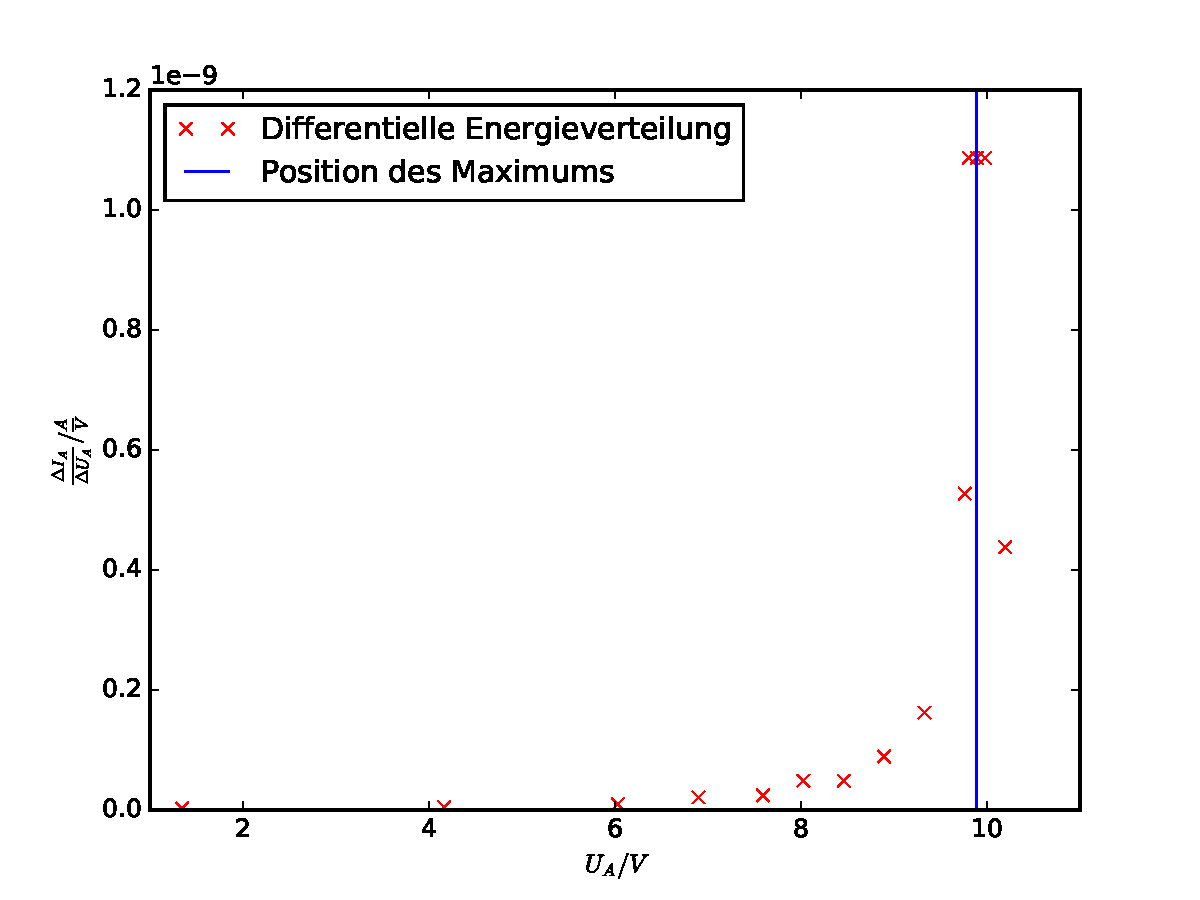
\includegraphics[height = 7cm]{plots/8a1plot.pdf}
  \caption{Differentielle Energieverteilung bei 296,35 \si{\kelvin}}
  \label{fig:8a1p}
\end{figure}

  \begin{figure}
    \centering
    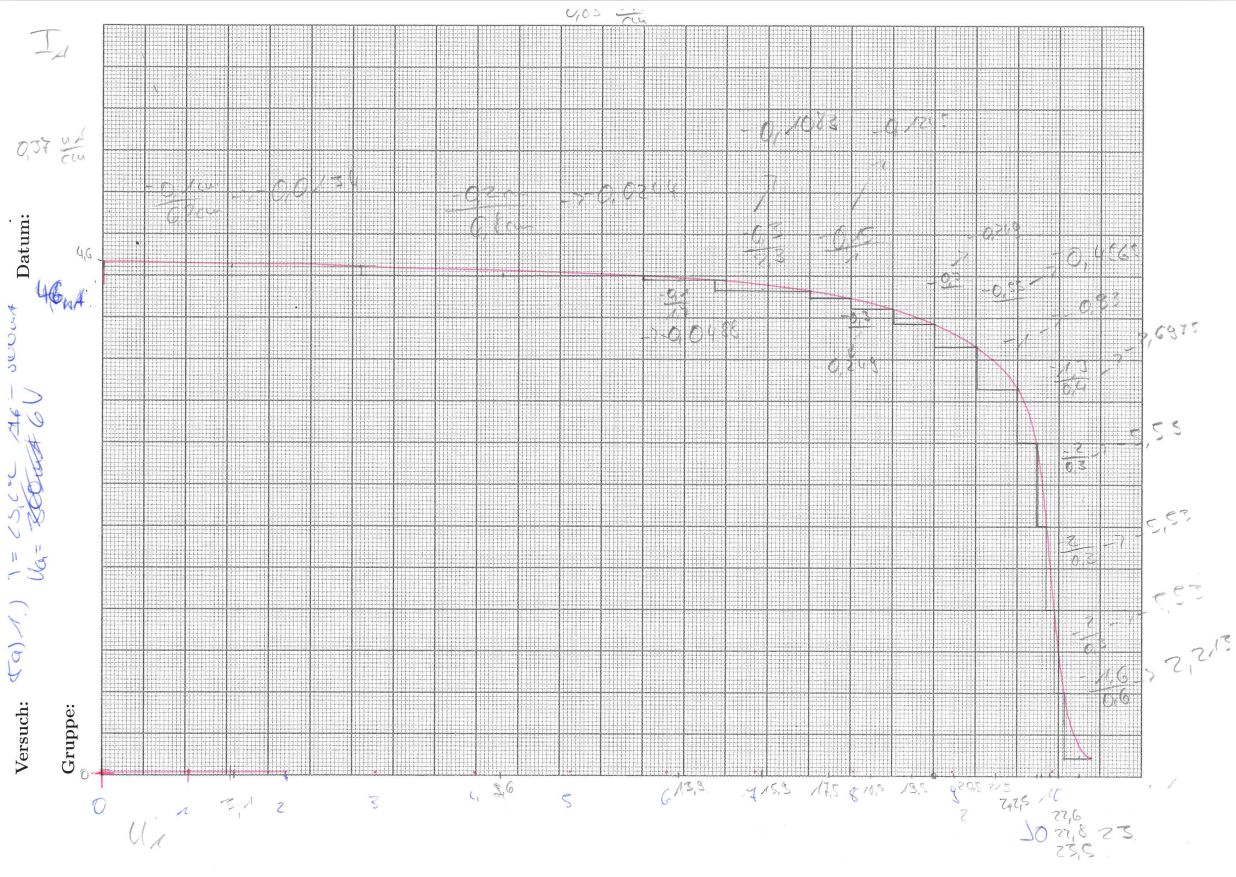
\includegraphics[height=7cm]{8a1.png}
    \caption{Auffängerstrom in Anhängikeit von der Bremsspannung bei 293,35 K}
    \label{fig:8a1}
  \end{figure}



\begin{figure}
  \centering
  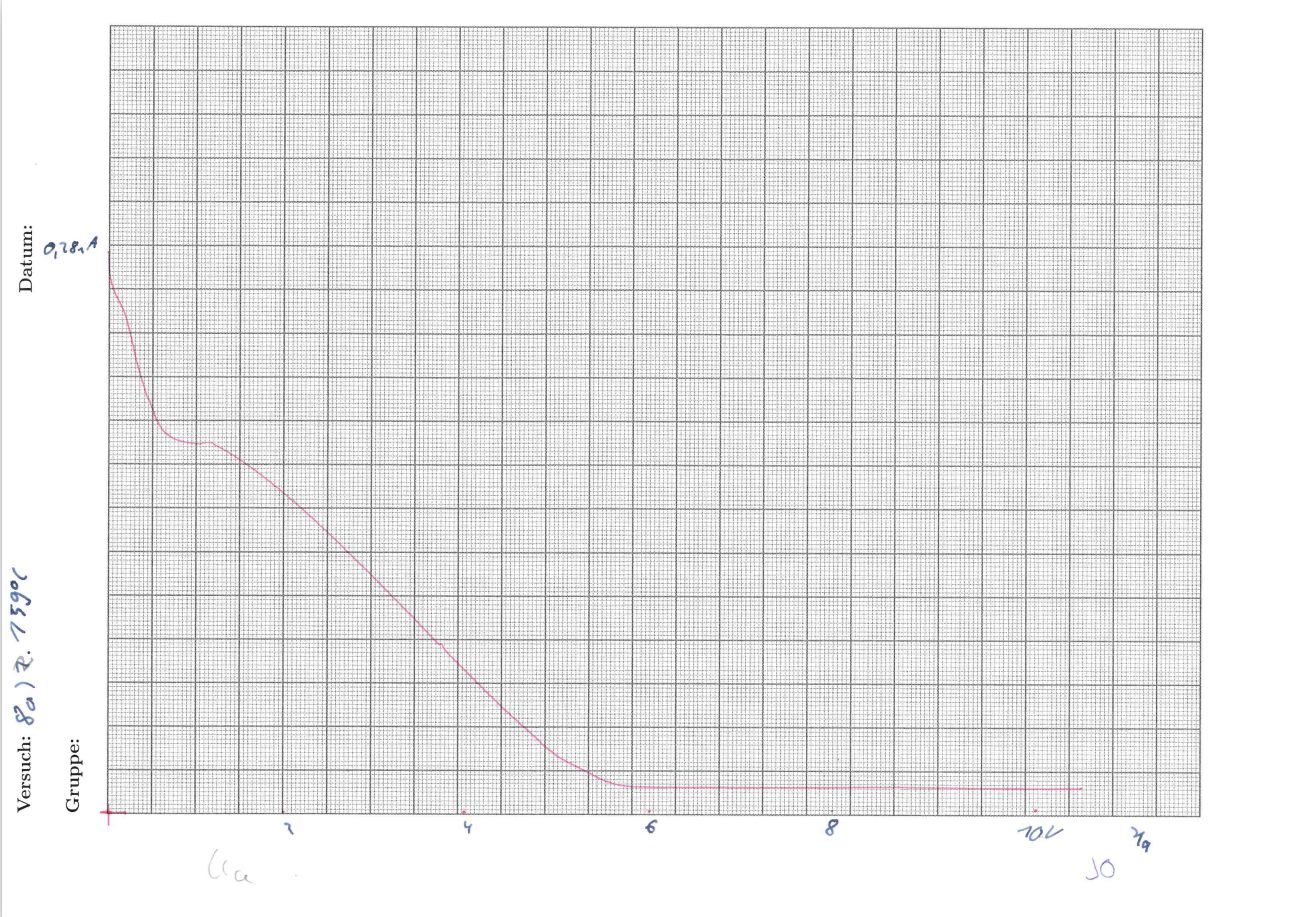
\includegraphics[height=7cm]{8a2.png}
  \caption{Auffängerstrom in Anhängikeit von der Bremsspannung bei 432,15 K}
  \label{fig:8a2}
\end{figure}


\subsection{Franck-Hertz-Kurve}
Die Abbildung \ref{fig:8b} zeigt die Franck-Hertz-Kurve. Die Abstande ziwschen
den Maxima wurden in der Abbildung vermessen, genauso wie die Skalenabstände.
Es wurde wieder auf Ablesefehler verzichtet. Danach
wurden die Skalenabstände gemittelt um einen Umrechnungsfaktor zu berechnen. Der
mittlere Skalenabstand beträgt ($3,91 \pm 0,07$) \si{\centi \meter}, der mittlere
Abstand zwischen den Maxima beträgt ($1,93 \pm 0,05$) \si{\centi \meter}. Daraus
ergibt sich der Umrechnungsfaktor ($2,56 \pm 0,05$) \si{\volt \per \centi \meter}
und daraus wiederum der mittlere Abstand der Maxima mit ($4,77 \pm 0,21$)\si{\volt}.
Aus dem mittleren Abstand der Maxima folgt dann die erste Anregungsenergie
$ U_1 = \left(4,77 \pm 0,21 \right) $\si{ \eV}. Mit der Gleichung
\begin{equation*}
  h\nu = E_1 - E_0 = U_1 \symup{e}
 \quad \text{und der Beziehung}\quad
   \lambda = \frac{c}{\nu}
\end{equation*}
lässt sich die Wellenlänge $\lambda $ des emittierten Lichtes berechenen, hier
bei bezeichet $h$ das Plancksche Wirkungsquantum \cite{scipy}, $ U_1 \symup{e}$ die
Anregungsenergie $U_1$ multipliziert mit der Elementarladung \cite{scipy},
 $\nu$ die Frequenz des emittierten Lichtes und $c$ die Lichtgeschwindigkeit \cite{scipy}.
Daraus ergibt sich, dass die Wellenlänge des emittierten Lichts
\begin{equation*}
  \lambda = \left( 260 \pm 11 \right) \si{\nano \meter}
\end{equation*}
beträgt.





\begin{figure}
  \centering
  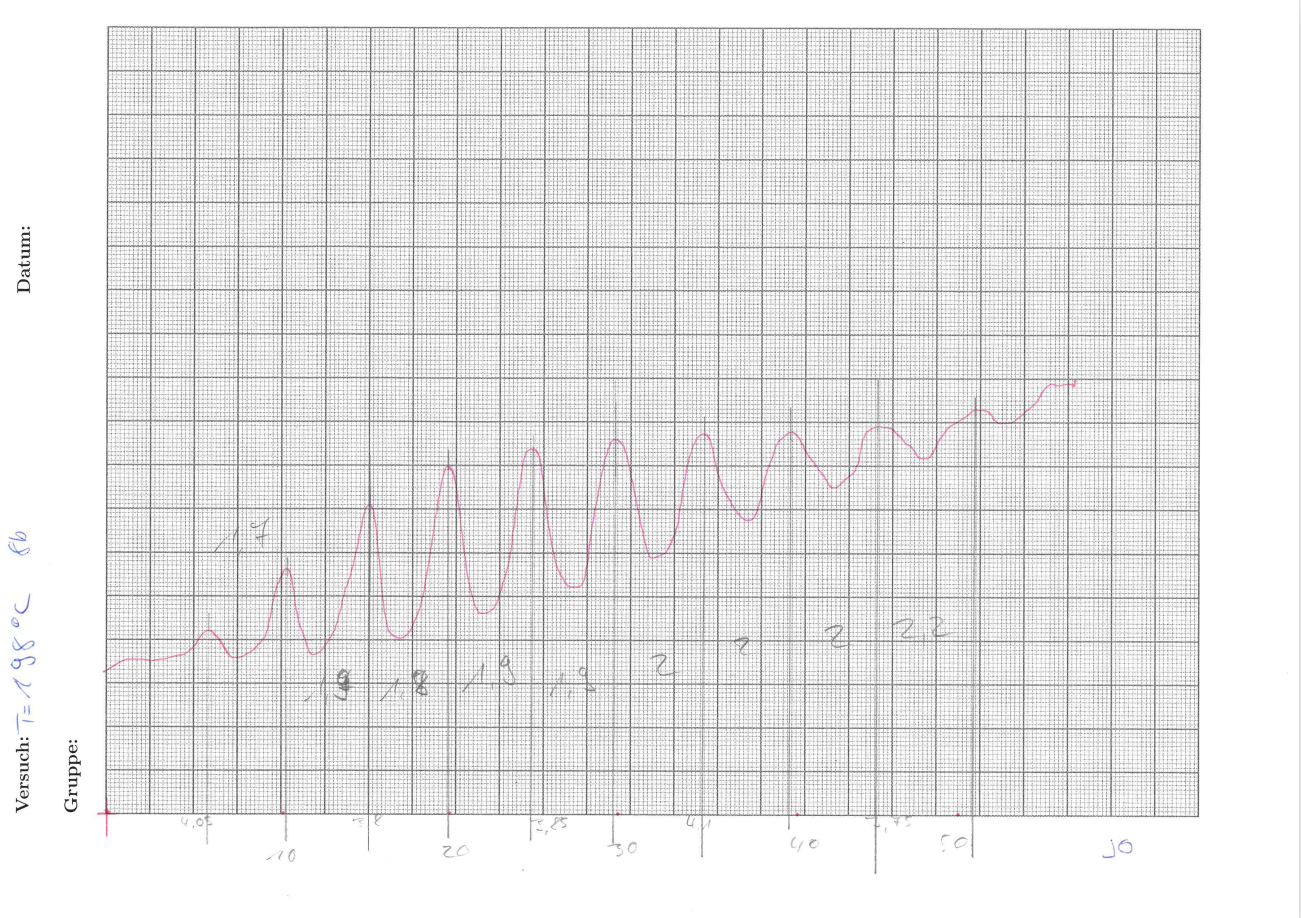
\includegraphics[height= 7cm]{8b.png}
  \caption{Franck-Hertz-Kurve bei 471.15 K}
  \label{fig:8b}
\end{figure}

\subsection{Ionisierung}
Zur Bestimmung der Ionisierungsspannung wird der Graph \ref{fig:8c} herangezogen und
an dessen Ausschlag wird eine Tangente bestimmt. Der Nulldurchlauf dieser Tangente
ist dann an der Stelle der Ionisierungsspannung plus das Kontaktpotential $K$. Die Ausgleichsgerade
\begin{equation*}
  f(x) = ax + b
\end{equation*}
wurde mit Scipy \cite{scipy} und Uncertainties \cite{uncertainties} bestimmt.
Dafür wurden die Werte erst aus dem Graph in Centimetern bestimmt, dann wurden
die Skalen gemittelt, ein Umrechnungsfaktor für die x-Achse bestimmt und die Werte
sowie die Ausgleichgerade in die Abbildung \ref{fig:io} eingezeichnet. Aus den
Werten $a$ und $b$ der Auslgeichsgeraden lässt sich dann rechnerisch der Wert
für den Nulldurchlauf bestimmen, dieser liegt demnach bei $ \left(8,5 \pm 0,5 \right)
\si{\centi \meter} $ was mit dem Umrechnungsfaktor $ \left(1,52 \pm 0,034 \right)
\si{\volt \per \centi \meter}$ ca. $\left( 12,9 \pm 0,8 \right) \si{\volt}$ entsprechen würde.
Daraus folgt dann, dass die Ionisierungsspannung bei $\left(11,8 \pm 0,8 \right) \si{\volt}$
liegt.
Alle Werte dazu sind in der Tabelle \ref{tab:iotab} dargestellt.
\begin{table}
  \centering
  \sisetup{round-mode = places , round-precision = 2}
  \begin{tabular}{S[scientific-notation = fixed, fixed-exponent = 0, round-precision =1] S[scientific-notation = fixed, fixed-exponent = 0, round-precision =1] S[scientific-notation = fixed, fixed-exponent = 0]@{$ \; \pm$} S[scientific-notation = fixed, fixed-exponent = 0]}
    \toprule
    $ x $ / \si{\centi \meter} & $y$ / \si{\centi \meter} & \multicolumn{2}{c}{$U_B \pm \Delta U_B / \si{\volt}$} \\
    \midrule
    7.400000000000000355e+00 & 0.000000000000000000e+00 & 1.125205576066159630e+01 & 2.514431713434237547e-01\\
    9.400000000000000355e+00 & 1.199999999999999956e+00 & 1.429315191219175674e+01 & 3.194007852200247966e-01\\
    1.140000000000000036e+01 & 2.600000000000000089e+00 & 1.733424806372191895e+01 & 3.873583990966257828e-01\\
    1.340000000000000036e+01 & 4.799999999999999822e+00 & 2.037534421525207762e+01 & 4.553160129732268246e-01\\
    1.540000000000000036e+01 & 7.200000000000000178e+00 & 2.341644036678223983e+01 & 5.232736268498278109e-01\\
    1.739999999999999858e+01 & 1.030000000000000071e+01 & 2.645753651831239850e+01 & 5.912312407264287417e-01\\
    1.939999999999999858e+01 & 1.350000000000000000e+01 & 2.949863266984255716e+01 & 6.591888546030297835e-01\\
    1.969999999999999929e+01 & 1.394999999999999929e+01 & 2.995479709257208256e+01 & 6.693824966845199897e-01\\
    \bottomrule
  \end{tabular}
  \caption{Werte der Ionisierungsspannung im Überblick}
  \label{tab:iotab}
\end{table}

\begin{figure}
  \centering
  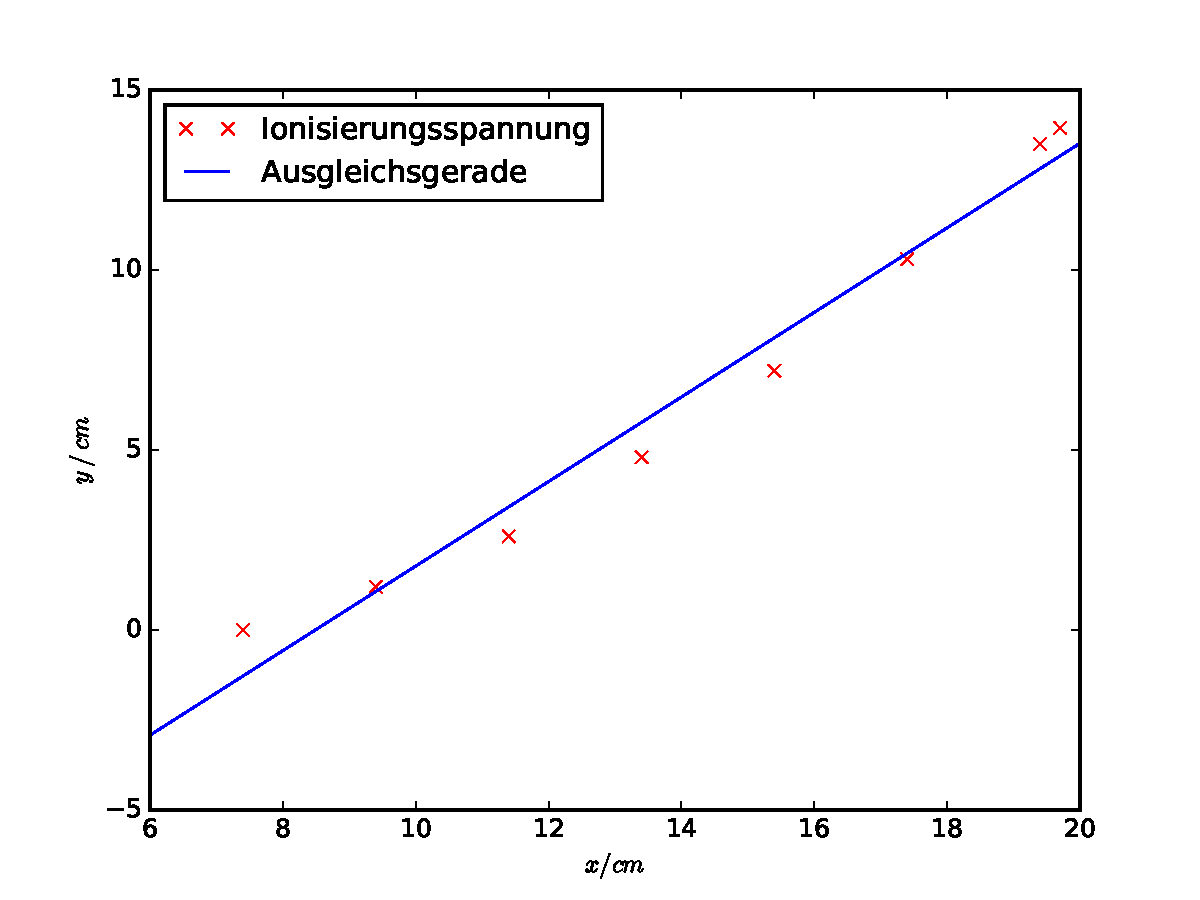
\includegraphics[height=7cm]{plots/8cplot.pdf}
  \caption{Ionisierungsspannung}
  \label{fig:io}
\end{figure}

\begin{figure}
  \centering
  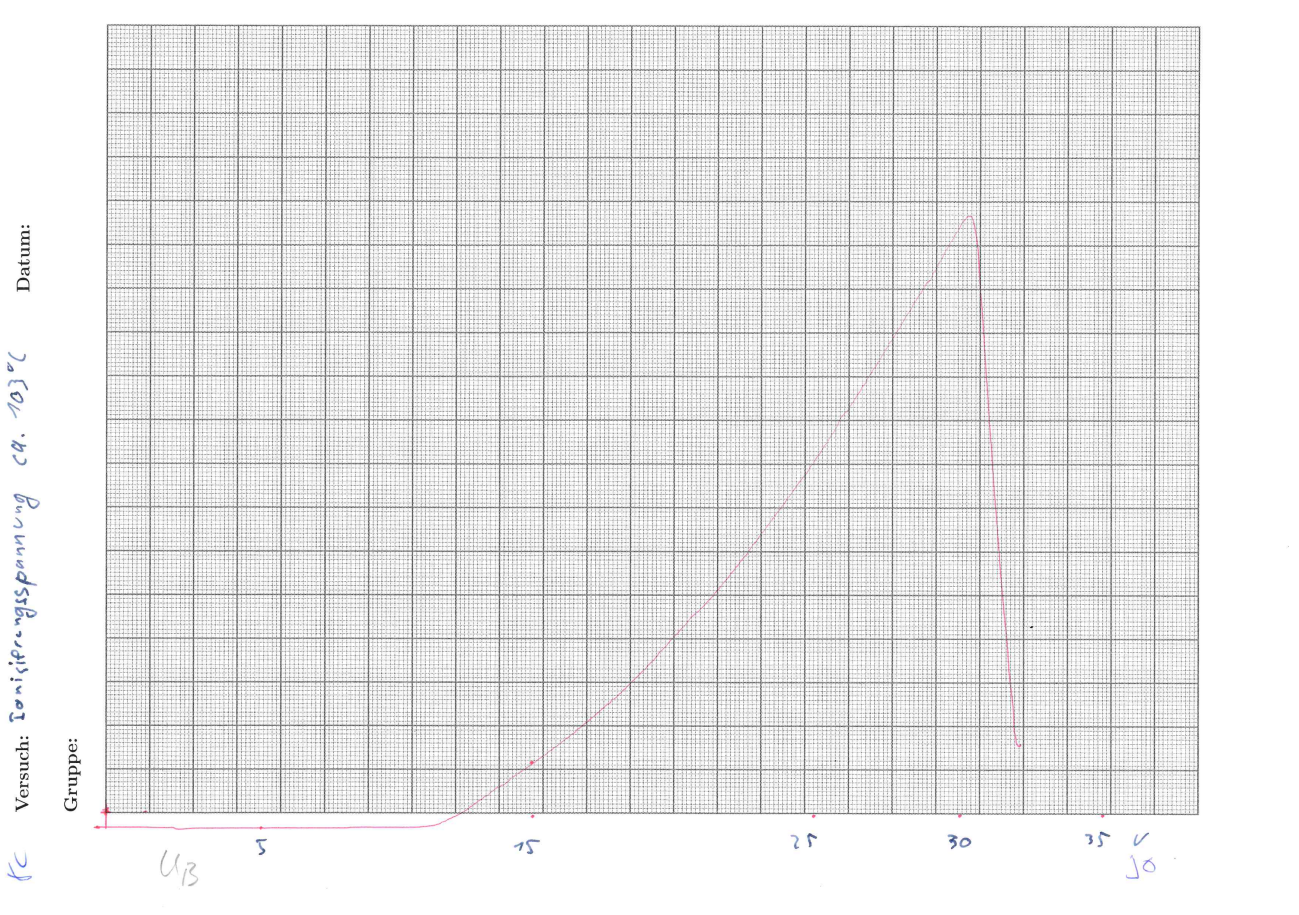
\includegraphics[height=7cm]{8c.png}
  \caption{Ionisierungspannung von Hg bei 376.15 K}
  \label{fig:8c}
\end{figure}
